\par The Large Hadron Collider (LHC)~\cite{Bruning:2004ej} is a 27 km-long underground 
syncrotron designed to accelerate and collide protons. For this reason, it is also 
referred to as an {\it accelerator}. It is located in a tunnel on the border of 
France and Switzerland, in which the Large Electron-Positron (LEP) 
collider~\cite{Myers:1991ym} once sat. Designed to accelerate
beams of protons to a maximum energy of 7~\TeV\ and to collide them at a total center-of-mass
collision energy (\sqs) of 14~\TeV, it is the largest accelerator ever built 
and collides the most energetic sub-atomic particles to date.

\par The fundamental principles on which an accelerator operates are complex. Reference~\cite{Wiedemann:1083415}
provides a detailed introduction to such principles. 
For a syncrotron built in a tunnel such as the LHC, particles are constrained in the circular path by
 dipole magnetic fields pointed in and out of the ground. Deviations in the directions 
parallel to the dipole magnetic fields are controlled by quadrupole magnetic fields. In other words, 
a series of dipole magnets is used to control circular motion, and a series of quadrupole magnets is 
used to focus the particles in a narrow aperture. Acceleration of particles is handled by electric fields 
pointing in the same direction as the particles' direction. In a circular arrangement such as in a syncrotron, 
these fields cannot be produced by a direct current voltage because the particles will get no overall 
acceleration over one cycle. Rather, an alternating voltage is used so that while the particles are accelerated 
at selected points in the circle, they do not decelerate at other points in the circle. These alternating 
fields are provided by radio-frequency (RF) cavities, whose frequency must always be an integer 
multiple of the particle revolution frequency. This arrangement causes particles of similar energies to 
group together, forming bunches of particles rather than a homegenous beam of particles.    

\par The LHC is part of a series of connected particle accelerators that make up the {\it accelerator 
complex}, shown by the schematic in Figure~\ref{fig:lhc}. First, hydrogen atoms are 
stripped of their electrons by an electric field in the Linear Accelerator
 2 (Linac2)~\cite{benedikt2004lhc}. The resultant protons are accelerated 
by alternating  electric fields due to an RF cavity arrangement in the Linac2. 
This splits the beam into multiple bunches of protons that eventually 
emerge from the other end of the Linac2 at 50~\MeV\ into the Proton Syncrotron Booster (PSB)~\cite{benedikt2004lhc}.  
The PSB uses superconducting dipole and quadrupole magnets to direct the proton bunches in a circular path 
and focus the beam into an aperture respectively. It also uses an RF cavity 
arrangement to accelerate the protons and split the beam even further. 

\par Protons emerge from the PSB at 1.4~\GeV\ into the Proton Syncrotron (PS)~\cite{benedikt2004lhc}. The PS is slightly 
larger than the PSB but the magnet and RF cavity arrangement is similar. The beam is fed into the
 Super Proton Syncrotron (SPS)~\cite{benedikt2004lhc}. The SPS further splits the proton beam, 
accelerates the protons to 450~\GeV\ and injects them into the LHC, which finally ramps their 
energy to 7~\TeV. During Run I, the LHC ramped protons to 4~\TeV\ and during Run II it ramped 
them to 6.5~\TeV.\footnote{Run I and Run II are defined in the Introduction}  

\par The LHC achieves this acceleration through the use of higher-frequency RF cavities. The protons are 
also kept in the circular tunnel and focused by stronger dipole and quadrupole superconducting magnets respectively.
More specifically dipole superconducting magnets, with a current of 11850~A, provides a 8.33~T peak magnetic field. Superconducting 
quadrupole magnets, with a current of 11870~A, provide a 6.85~T peak magnetic field. 400~MHz RF cavities are used 
for acceleration, with a total voltage of 16~MV. This setup produces a beam, which is 
made up of 2808 bunches of length 7.55~cm, of radius \SI{16.7}{\micron} upon collision.  
With this nominal setup, on average there are $1.15\times 10^{11}$ protons in each bunch.
During Run I each beam comprised 1374 bunches, and the number of protons in each bunch ranged 
between $1.6\to 1.7\times 10^{11}$. During Run II each beam comprised 2076 bunches, and the number of protons 
in each bunch was about $1.18\times 10^{11}$. The number of collisions during each bunch crossing 
is known as {\it in-time pileup}, while the number of overlapping collisions from separate 
bunch crossings is known as {\it out-of-time pileup}. During Run I and Run II pileup of 40 was 
observed; the design pileup is 20. Table~\ref{tab:lhcParas} summarizes these parameters.  


\begin{table}[!h]
\centering
   \begin{tabular}{|l|ccc|}
\hline
 Parameter           								& Run I Value    & Run II Value & Design Value \\
\hline\hline
Beam Energy [\TeV]   								&          4     &  	6.5       &    7         \\
Bunch spacing [\SI{}{\nano\second}] & 				50 		 & 		25 				& 	25 				 \\
Protons per bunch										&\num{1.7e11}    & \num{1.18e11}& \num{1.15e11}\\
Collisions per bunch crossing       &  40            &  40          & 20    \\ 
\hline
   \end{tabular}
\caption{Values of some of LHC parameters during Run I (2010$\to$2012) and Run II (2015$\to$16). The design 
values are also listed.}
\label{tab:lhcParas}
\end{table}

\par Red arrows in Figure~\ref{fig:lhc} illustrate the proton beam passage through
this accelerator complex.  

\begin{figure}[!h]
	\centering
   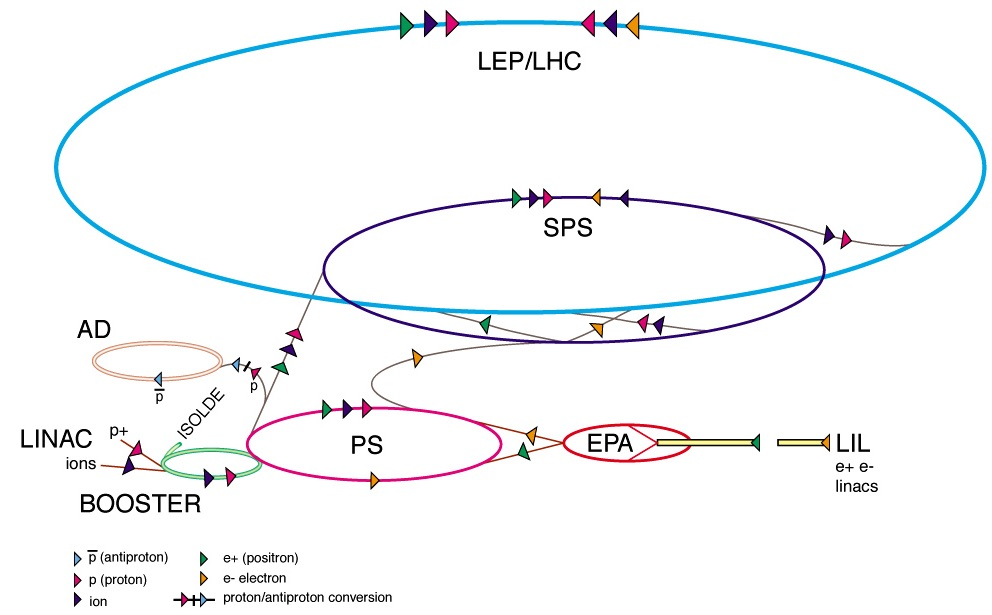
\includegraphics[width=\textwidth]{figures/lhc-pho-1991-001.jpg}
	\caption{The accelerator complex for the LHC. Apart from accelerating protons, the LHC 
					is also used to accelerate and collide heavy ions. Arrows represent the particles' 
					pathway from production to collision, with a key at the bottom left indicating 
					the type of particle}
	\label{fig:lhc}
\end{figure}

\par In addition to accelerating protons, the LHC is also accelerates heavy 
ions. Passage of such ions is illustrated by arrows in Figure~\ref{fig:lhc} as well, as defined 
in the key. Collisions in the LHC are done at 4 points, at which high resolution detectors are built:
ATLAS~\cite{1748-0221-3-08-S08003} on which the work for this thesis was done, 
CMS~\cite{Chatrchyan:2008aa}, LHCb~\cite{Amato:1998xt} and ALICE~\cite{1748-0221-3-08-S08002}.


\par A major LHC goal is to produce rare physics processes in abundance through proton-proton (\pp) 
collisions. The number of events per second $N_{process}$ during which such rare process are produced  
is proportional to the cross-section $\sigma_{process}$ of the process in question: 

\begin{equation}
N_{process} = L\sigma_{process}
\label{eq:lumi}
\end{equation}

where $L$ is a property called {\it luminosity}. The integral of luminosity over a time 
of LHC operation $T$ is usually quoted: 

\begin{equation}
\mathcal{L} = \int_0^{T} L dt. 
\label{eq:intL}
\end{equation}

From Equation~\ref{eq:lumi} $N_{process}$ is optimized by either increasing $L$, $\sigma_{process}$, 
or both. $\sigma_{process}$ is directly proportional to \sqs, which is in turn directly proportional to
 beam energies. To increase $\sigma_{process}$, two options are available:
\begin{enumerate} 
\item the superconducting dipole magnets used to control the beam's circular path could 
be upgraded while keeping the circular path constant;
\item or the radius of the LHC could be increased.
\end{enumerate}
 Superconductivity in general is a very 
active area of modern research and the LHC has exploited the most current results. 
 The second option is under serious consideration~\cite{Arkani-Hamed:2015vfh} 
for future generation colliders. A more feasible strategy to optimize $N_{process}$ 
would be to optimize $L$ whose parameters are shown in Equation~\ref{eq:lDef}, rather than $\sigma_{process}$.  

\begin{equation}
L \propto \frac{N^2_bn_bf_{rev}\gamma_r}{4\pi\epsilon_n\beta^*}
\label{eq:lDef}
\end{equation} 

$N_b$ is the number of protons in a bunch, $n_b$ is the number of bunches in a beam, 
$f_{rev}$ is the beam revolution frequency, $\gamma_r$ is the relativistic gamma factor at the 
collision point, $\epsilon_n$ is the normalized transverse beam emittance and $\beta^*$ 
is the beta function at the collision point.
Beam emittance is a measure of the beam size in angular and position phase space. At the LHC
it is measured in~\SI{}{\um\radian} and it is not always constant during beam acceleration. 
In contrast, the normalized beam emittance, $\epsilon_n$, is always constant and therefore 
more useful in optimizing $L$. $\beta^*$ is the width of the beam divided by its emittance. 
So for low $\beta^*$ and $\epsilon_n$ the chance of protons colliding increases, in turn increasing $L$.  

\par As the proton beam traverses the collider ring, it forms a current and hence a magnetic field 
around itself. Upon bunch collision, the colliding protons may be deflected by fields induced 
by the magnetic fields due to each beam. The beam crossing angle is designed to be kept at 
\SI{285}{\micro\radian} to tune the protons against these deflections. A larger crossing 
angle would lead to emittance growth and beam instabilities. 

\par During Run I, the LHC reached $L = \num{7.7e33}\SI{}{\cm^{-2}\s^{-1}}$. During Run II, 
 reached $L = \num{1.2e34}\SI{}{\cm^{-2}\s^{-1}}$. Figure~\ref{fig:peakLumi} shows distributions 
of the peak luminosity during Run II (2016 data-taking period) and during Run I. 
At the end of Run I the LHC delivered 20.3~\ifb of data and by July 2016 during Run II 
%it had delivered 14.7~\ifb as shown in Figure~\ref{fig:lumiInt}.

\begin{figure}[!h]
\begin{subfigure}{0.5\textwidth}
   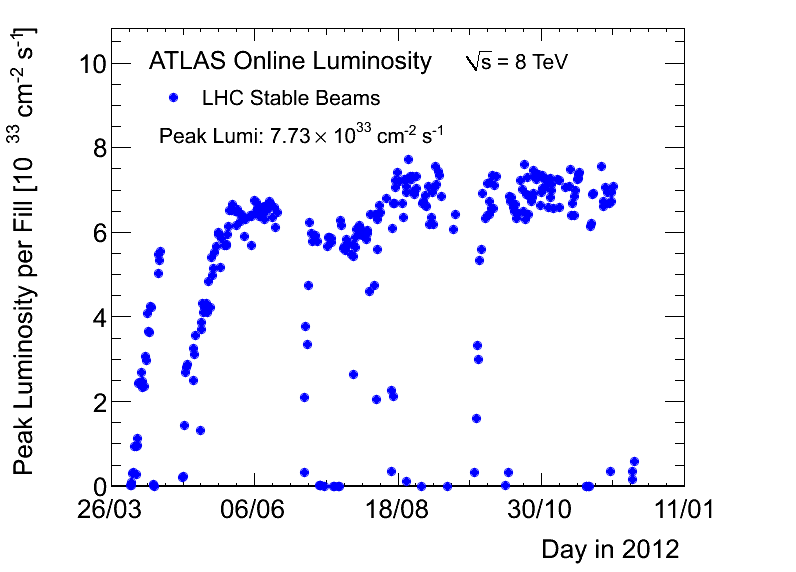
\includegraphics[width=\textwidth]{figures/peakLumiByFill2012.png}
	\caption{Run I. Taken from Ref~\cite{ATLAS:lumi2012}}
\end{subfigure} % 
\begin{subfigure}{0.5\textwidth}
   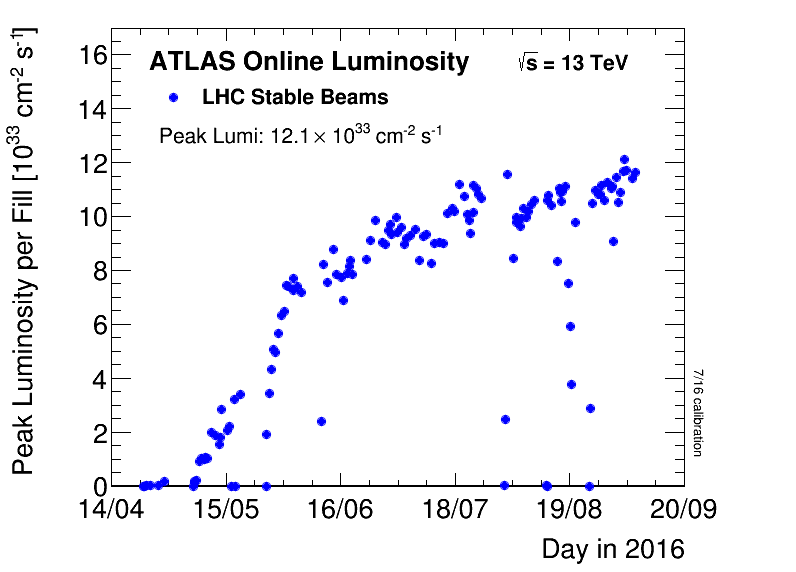
\includegraphics[width=\textwidth]{figures/peakLumiByFill.png}
	\caption{Run II. Taken from Ref~\cite{ATLAS:lumi}}
\end{subfigure}
	\caption{Peak luminosity from the LHC during Run I and Run II}
\label{fig:peakLumi}
\end{figure}

%\begin{figure}[!h]
%\centering
%   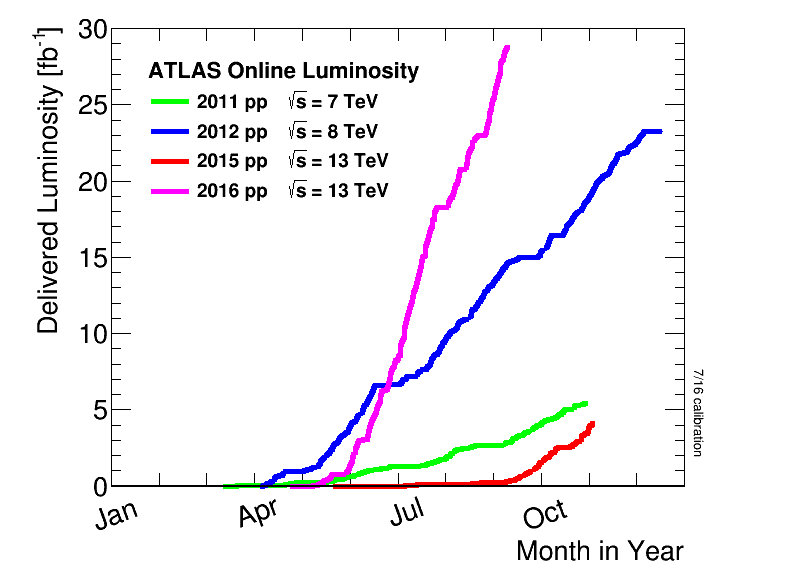
\includegraphics[width=0.5\textwidth]{figures/intlumivsyear.png}
%	\caption{Integrated luminosity from the LHC during Run I and Run II. Taken from Ref~\cite{ATLAS:lumi}}
%\label{fig:lumiInt}
%\end{figure}
